\documentclass{article}
\usepackage[utf8]{inputenc}
\usepackage[margin=1in]{geometry}
\usepackage{amsmath}
\usepackage{gensymb}
\usepackage{hyperref}
\usepackage{graphicx}
\graphicspath{ {./images/} }

\hypersetup{
    colorlinks=true,
    linkcolor=blue,
    filecolor=magenta,      
    urlcolor=blue,
}

\title{[ECS 175] Report}
\date{12/07/2020}
\author{Group 8}

\begin{document}

\maketitle

\section*{Introduction (1 page)}
\subsection*{Problem Statement}
Our project aims to predict whether a given YouTube video is classified as "trending" or "non-trending" by Google. We did this by creating our own dataset through Google's YouTube Data v3 API which contained present and historical information about a video. This problem is a binary classification problem as we are predicting one of two classes. Thus, we implemented prediction with both Neural Network and Logistic Regression models, and compared the two to find the best model overall. In addition, we expanded the problem scope from simple binary classification to multiclass classification by utilizing clustering. Although this does not directly solve our original problem, it gave us avenue to predict a YouTube video's success.

\subsection*{Group Members}
\subsubsection*{Data Gathering Sub-Group:}
- \textbf{Contribution:} Wrote and manage script to get data from Youtube Data API \\
- \textbf{Members:} Ted Kahl, Rohail Asad
\subsubsection*{Data Processing Sub-Group:}
- \textbf{Contribution:} Processed data from API into effective dataset \\
- \textbf{Members:} Phalgun Krishna, Prajwal Singh, Seth Damany
\subsubsection*{Machine Learning Sub-Group:}
- \textbf{Contribution:} Created and optimized ML models \\
- \textbf{Members:} Cameron Yuen, Owen Gao, Theresa Nowack, Trevor Carpenter
\subsubsection*{Documentation and Web App Sub-Group:}
- \textbf{Contribution:} Created web app and managed documentation \\
- \textbf{Members:} Josh McGinnis, Keith Choung, Nikhil Razdan, Thu Vo
\subsubsection*{Group Leader:}
- \textbf{Contribution:} Organized milestones and facilitated communication \\
- \textbf{Members:} Nikhil Razdan

\subsection*{Project Links}
- \textbf{GitHub:} \url{www.github.com/nsrazdan/ECS-171-Group8} \\
- \textbf{YouTube Data v3 API:} \url{developers.google.com/youtube/v3/} \\
- \textbf{Original Kaggle Dataset:} \url{www.kaggle.com/datasnaek/youtube-new} \\

\section*{Literature Review (1 page)}
\subsection*{Primary Source}

\quad In looking at other sources with similar topics, we found that various studies defined popularity differently. Our group used YouTube’s trending feature as our popularity metric. Another similar study from Stanford used videos’ view counts instead. This study, titled \textit{YouTube Videos Prediction: Will this video be popular?}, analyzed the topic of predicting a video’s success from the perspective of a YouTube content creator. Instead of a simple binary classification “trending?” target variable like our group utilized, the researchers Li, Kent, and Zhang from Stanford divided the classification into 4 disjoint categories: non-popular, overwhelming praises, overwhelming bad views, and neutral videos. They used multi-class classification to analyse and quantify the success of a video in seeing whether it was reacted to positively or negatively. The researchers used similar attributes as our group, such as view count and duration. However, they also included an important attribute that fits in line with their ‘YouTuber’ point of view: time gap. This takes into account the possibility that frequent and regular uploads are favored by YouTube’s recommendation/trending selection process as opposed to a sporadic upload schedule. By using the YouTube dataset from Kaggle that inspired our project’s dataset, this particular research paper bears many similarities with our own.
\par Li, Kent, and Zhang found that extreme gradient boosting with attributes \{time gap, category, and description\} produced the best results with the highest F1 score out of the other methods they tried. Instead of downsampling to account for the imbalanced data, the team of researchers added class weights. They report that the highest indicators of popularity (eg. view count) are a video’s category, description and time gap. When concluding their research paper, they note that the issue of overfitting remains a concern. To improve, they suggested adding more attributes such as video thumbnails and subtitles, as well as expanding the dataset for a more balanced set of videos. This particular source provides a clear framework to position our own project. Importantly, we added a large set of non-trending videos in our data to give it enough information to classify trending status. \smallskip

\href{http://cs229.stanford.edu/proj2019aut/data/assignment_308832_raw/26647615.pdf}{http://cs229.stanford.edu/proj2019aut/data/assignment\_308832\_raw/26647615.pdf}

\subsection*{More Related Works}

\quad The Towards Data Science article by Arvind Srinivasan, "YouTube Views Predictor," discussed a model that utilizes very interesting and unique variables our group had not thought of in its prediction model. Although the two projects differ slightly given that the “YouTube Views Predictor” model predicts the number of views a YouTube video will get and ours predicts whether a YouTube video will become trending, many of our features remain the same. However, the creators included other features such as a “Clickbait Score,” a NSFW Score,” and whether a YouTube video’s title contained words related to common or popular YouTube genres to better determine its popularity. \smallskip

\href{https://towardsdatascience.com/youtube-views-predictor-9ec573090acb}{https://towardsdatascience.com/youtube-views-predictor-9ec573090acb} \bigskip

\par Clustering was a method that the Machine Learning team would like to have implemented in order to discover groups of videos which would allow us to further focus the scope of our predictions of trendability. \textit{Clustering the Unknown - The Youtube Case} by Amit Dvir, Angelos K. Marnerides, Ran Dubin, Nehor Golan did exactly that and took 100,000 video streams to cluster unknown videos based on their title and grouped them with the use of K-means clustering and the help of NLP formulations and Word2Vec. They were able to identify many unique clusters that had their own traits purely based on video title and not by any other traits given by the metadata of youtube videos. \smallskip

\href{https://www.researchgate.net/publication/332376497_Clustering_the_Unknown_-_The_Youtube_Case}{https://www.researchgate.net/publication/332376497\_Clustering\_the\_Unknown\_-\_The\_Youtube\_Case} \bigskip


\textit{Trending Videos: Measurement and Analysis} studies Youtube’s trending videos in terms of viewership lifecycle and other basic statistics of their content. Researchers also collected a list of non-trending videos in order to do comparative analysis between trending and non-trending videos. To distinguish the difference between trending and non-trending videos, they conducted comparative analysis on (1) the standard video feeds, which provide basic statistics of the videos and (2) video uploaders’ profile. Moreover, the study used Granger Causality (GC), which provides deeper insight onto viewership pattern, to derive directional-relationships among trending-video time-series. The study concluded that there’s a distinct difference between the statistical attributes of trending and non-trending videos. GC measurement confirms the directional relationship between trending videos and other videos in the dataset, and among different categories of trending videos. \smallskip

\href{https://www.researchgate.net/publication/266262149_Trending_Videos_Measurement_and_Analysis}{https://www.researchgate.net/publication/266262149\_Trending\_Videos\_Measurement\_and\_Analysis} 

\subsection*{References}
\begin{enumerate}
  \item Li, Yuping, et al. Stanford, 2019, \textit{YouTube Videos Prediction: Will This Video Be Popular?} 
  \item Srinivasan, Aravind. “Youtube Views Predictor.” Medium, Towards Data Science, 17 Dec. 2017, \href{https://towardsdatascience.com/youtube-views-predictor-9ec573090acb}{https://towardsdatascience.com/youtube-views-predictor-9ec573090acb}
  \item Dvir, Amit, et al. Arial University \& Lancaster University, 2019, \textit{Clustering the Unknown - The Youtube Case}
  \item Barjasteh, Iman, and Ying Liu. Michigan State University, \textit{Trending Videos: Measurement and Analysis}
\end{enumerate}


\section*{Dataset Description (0.5 pages)}
\pagebreak
\section*{Proposed solution and experimental results (4-5 pages)}
\subsection*{Proposed Solution}

\quad As our initial task was one of binary classification, checking if a YouTube video is trending or not, we utilized primarily the YouTube definition of a “trending” video. This way, we could theoretically predict if a video would make it onto the trending chart that YouTube chooses on their own. In order to accomplish this, we first built two models, one logistic to predict the class that a video would fall into and the other a neural network.
\par Logistic regression is a good way to perform classification using probabilities and it is less sensitive to the prediction threshold and any outliers that may be in the data than linear regression is. We experimented with various combinations of hyperparameters, such as the ‘newton-cg’, ‘liblinear’, ‘sag’, ‘saga’, or ‘lbfgs’ solvers and the ‘l1’, ‘l2’, or ‘elasticnet’ penalties while fitting our model.  We found that the Limited-memory Broyden–Fletcher–Goldfarb–Shanno (LBFGS) solver with l2 penalty produced the best model with the highest accuracy (about 0.8451883).  Like the Newton method, LBFGS gives more accurate results, because it uses both the first and second derivatives of the likelihood function when updating the model’s weights, but it only uses an approximation of the second derivative, making it less computationally expensive than newton-cg.  L2 regularization prevents any of the weights from getting too large, giving too much influence to a single attribute and leading to potential over-fitting, while also stopping any of the weights from being minimized all the way down to zero (feature selection).

\begin{center}
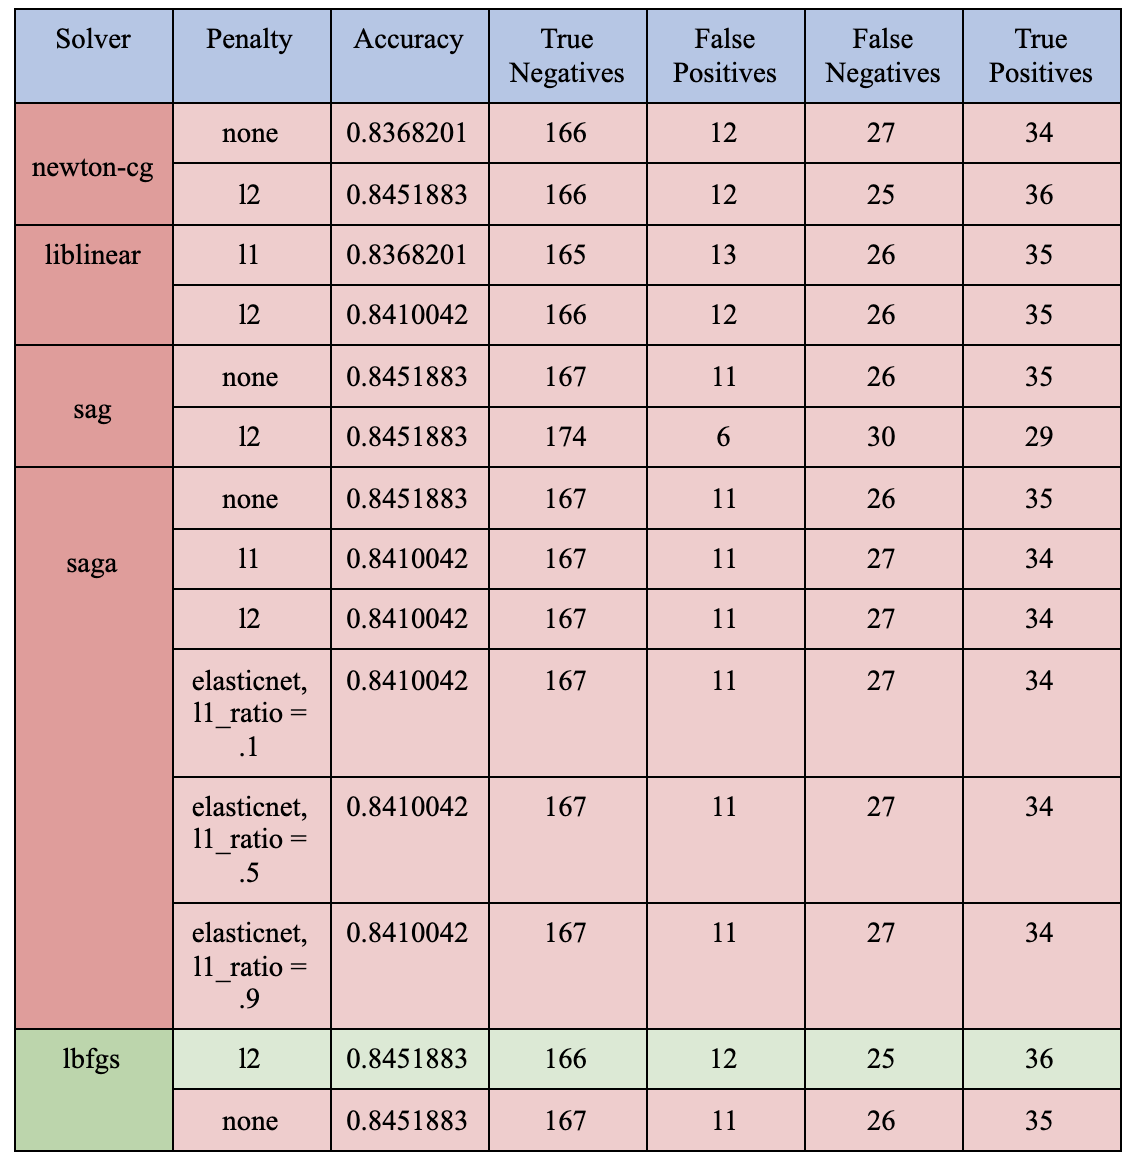
\includegraphics[scale=.5]{solver_results.png}\\
\end{center}

\quad From here, we still faced a binary classification problem, but wanted to try fitting it to a more complex model to see if we could obtain better prediction results.  Artificial Neural Networks (ANN) can model much more complex relationships than logistic regression can.  The model with the greatest precision that we found was a five-layer ANN with thirty-six nodes in the input layer, twenty nodes in the first hidden layer, thirty in the second hidden layer, twenty in the last hidden layer, and a single node in the output layer for our binary classification of trending or not trending.  We used the Adam optimizer because it uses separate learning rates for each weight which it updates based on both the average and the variance of the recent rate of change for that weight.  This makes it a better option for handling larger amounts of data since it can adapt its learning as it goes to address the different behaviors and contributions of our different parameters.  We chose to use sigmoid activation functions because the sigmoid function provides a smooth gradient that does not jump between values and produces an output value that is bound between 0 and 1 which normalizes the output of each neuron. We used mean squared error as we found that it worked best with our data set. With mean squared error, the more data used, the less error there due to the average of the sum of squares being used. The learning rate of an ANN is the rate of which controls how much to change the model in response to the estimated error each time the model weights are updated. Finding the right learning rate is key to a successful and accurate model in that a learning rate that is too low will not produce enough positives and a learning rate that is too high will produce too many positives, i.e. false positives. We found that the value that produced a balance result was a learning rate of 0.005. An epoch is defined as a one cycle through the whole training dataset. We settled on 300 epochs. The batch size is a hyperparameter that controls the number of training data samples that are used. We settled on a batch size of 200.  Using different optimizers we got different values for accuracy, recall and precision. The following chart shows our findings. Again, we settled on using the Adam optimizer. 
\begin{center}
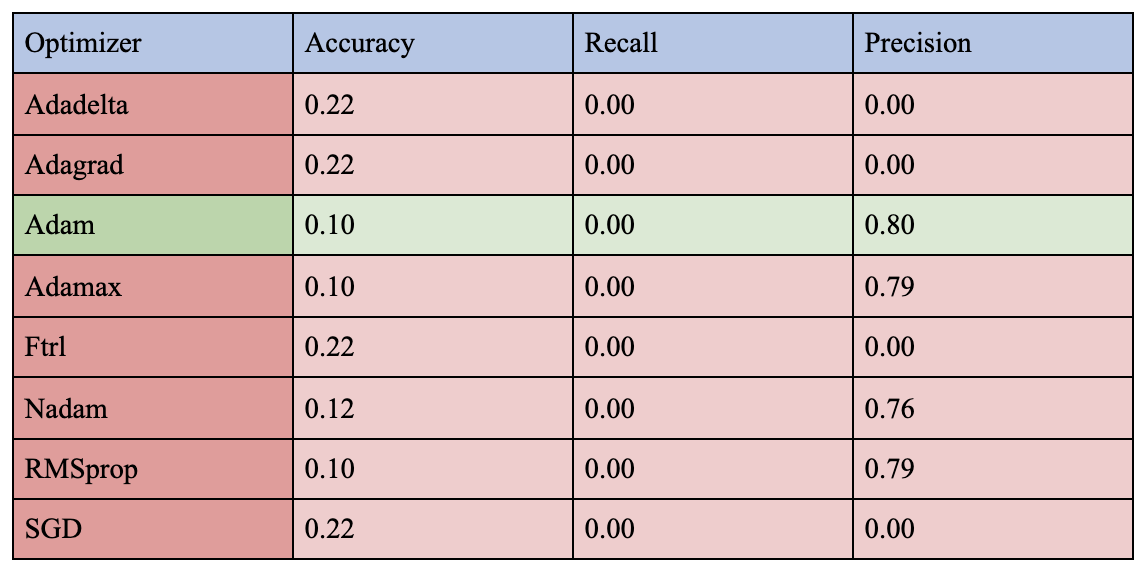
\includegraphics[scale=.55]{optimizer_results.png}\\
\end{center}

\subsection*{Experimental Results}

\quad The performance of the logistic regression model is summarized in the confusion matrix shown in the figure below. A false positive is the least likely to be generated by our model while a false negative has roughly a 10.5\% chance of being generated. 

\begin{center}
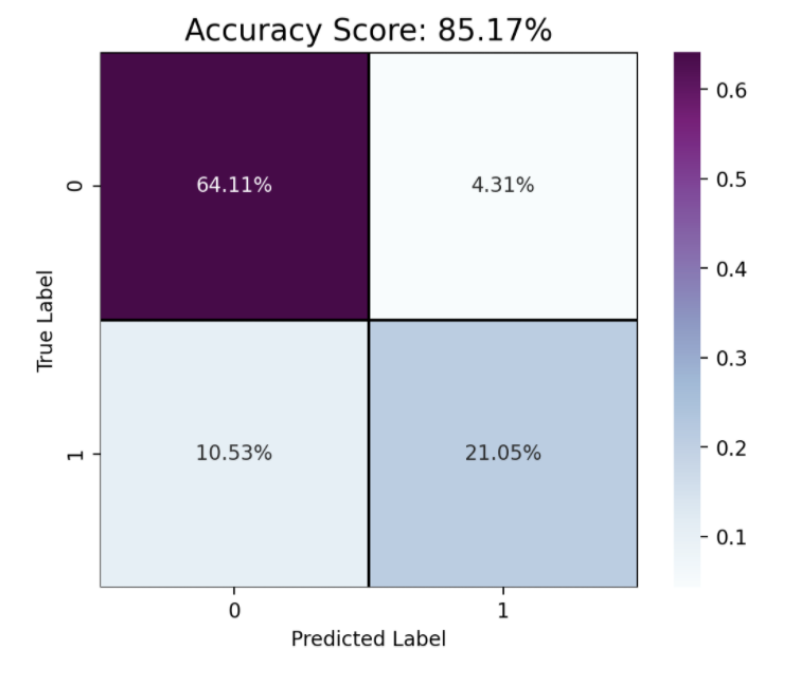
\includegraphics[scale=.65]{confusion_matrix.png}\\
\end{center}

\quad The receiver operating characteristic (ROC) curve is provided in Figure 2. This ROC curve shows that our generated model performs much better than random guessing. The rates of true positives and false positives are shown for all thresholds from zero to one. Our model uses a threshold of 0.5 which may be identified on the graph when the x value is 0.0431. (reword this later)
 1: Confusion matrix generated by the Logistic Regression model with a threshold of 0.5.
 \begin{center}
 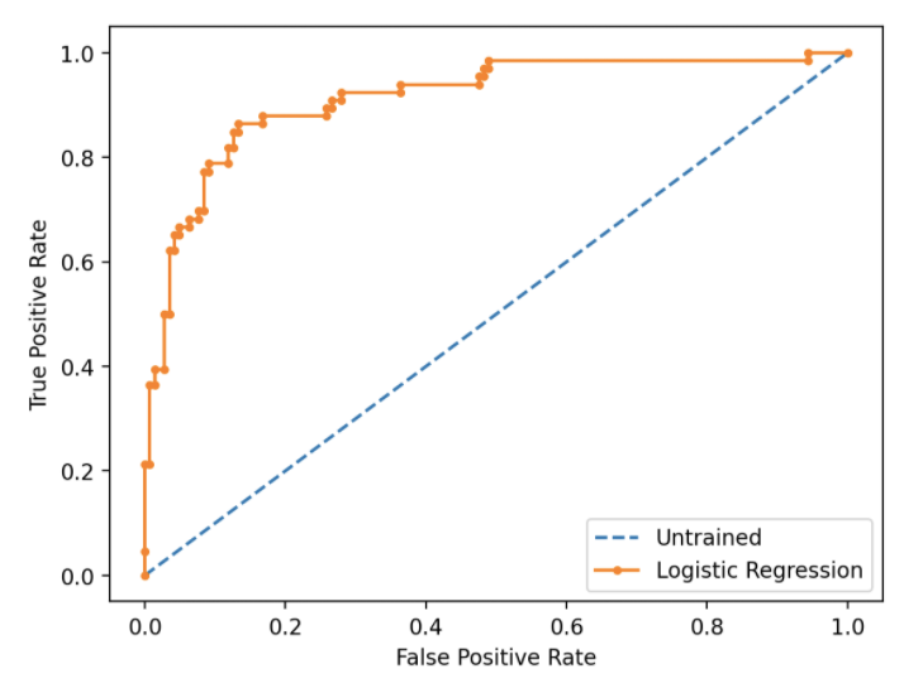
\includegraphics[scale=.65]{figure2.png}\\
 \textbf{Figure 2:} ROC Curve showing performance of the logistic regression model at various thresholds
\end{center}

\par The performance of the neural network model is shown in Figure 3. It can be seen that a false positive result is the least likely we are to encounter (5.74\%) while a false negative is the second least likely to be encountered (7.66\%).

\begin{center}
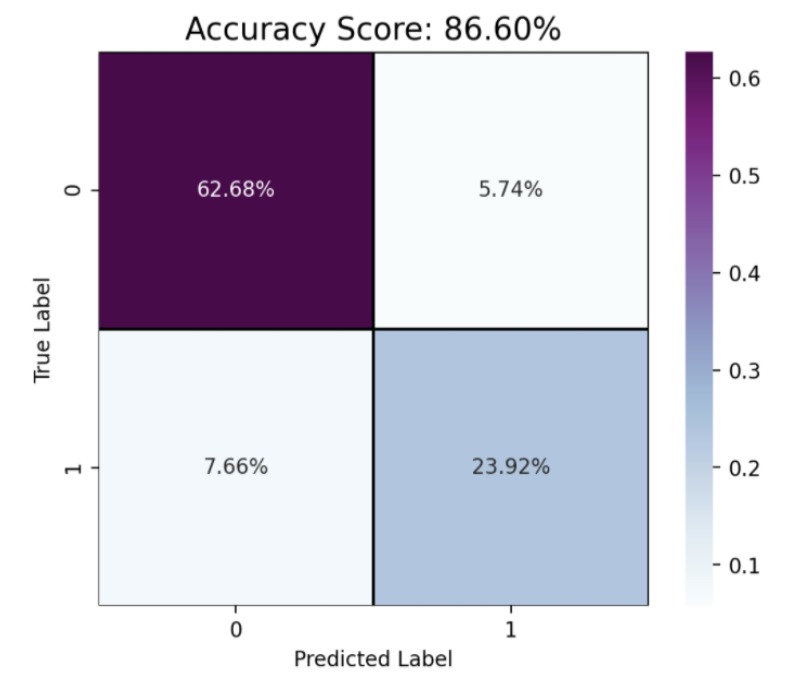
\includegraphics[scale=.65]{figure3.png}\\
\textbf{Figure 3:} Confusion matrix generated by the neural network model with a set threshold of 0.5.
\end{center}

\subsection*{Clustering}

\quad While we were developing the above models, we recognized some secondary issues with our initial problem. YouTube, being a large company run by Google, is constantly gathering data on videos at a rate and level extremely difficult to replicate. While we were able to get decent prediction values on our testing data, that was data resulting in weeks of gatherings. 
\par We began to ask what would be necessary to accurately predict based on a snapshot of a YouTube video. Removing all data that cannot be mined at a singular point in time would leave statistics about the video at that moment such as likes, views, comments, and other attributes of the video itself such as duration, title, and description. Predicting with only these momentary attributes however results in poor statistics for our testing data: \\

\textbf{Logistic Regression:} Accuracy: 0.742857 
\par \textbf{Neural Network:} Accuracy: 0.64 
\begin{center}
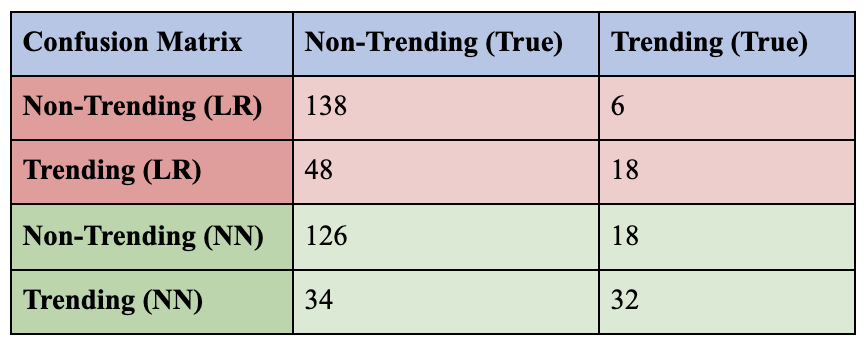
\includegraphics[scale=.7]{momentary_at.png}\\
\end{center}
\quad Clearly it is inaccurate to classify the trending algorithm with only a snapshot of a YouTube video. However, that does not mean it is impossible to classify videos in general. This is when we turned to unsupervised learning and clustering. Our flaw with predicting based on a snapshot was that we were trying to emulate an algorithm that takes into account time as a large factor, whereas we could not use that in a momentary prediction. But if we could cluster the data we did have based on momentary data into a self-defined number of clusters with the K-Means Clustering algorithm, we could predict the cluster a video would be in, and from that gather general data predictions about that video.
\par Using three labels instead of two, for example, on the data from before, would produce the following results: \\

\textbf{Logistic Regression:} Accuracy 0.9952380952380953
\par \textbf{Neural Network:} Accuracy 0.9571 
\begin{center}
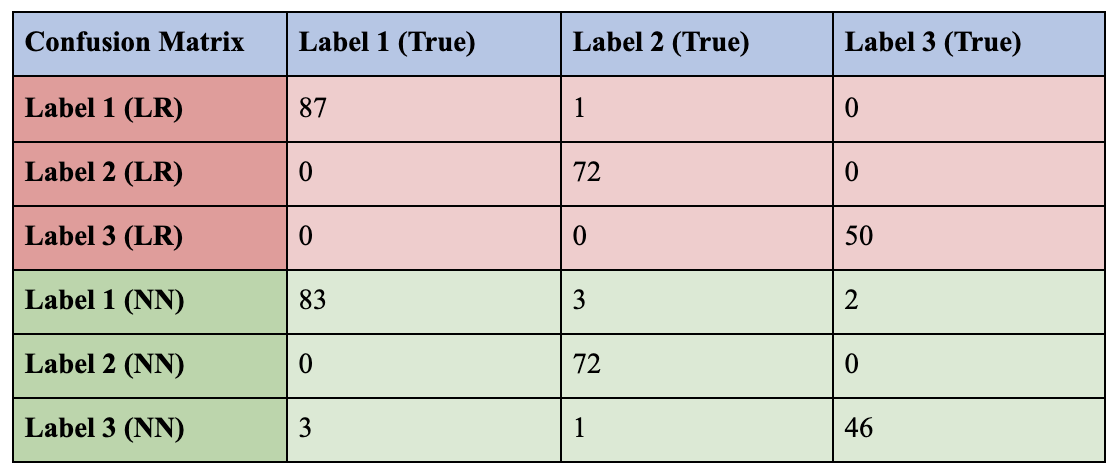
\includegraphics[scale=.7]{multi_label.png}\\
\end{center}
\quad Based on the data, we can see that adding an extra label instead of simply isolating trending videos from non-trending videos greatly increases the accuracy of a model. We utilized a WCSS graph to check the optimal cluster value if we were to cluster the data further as such and reported based on the elbow of the graph below that this value is greater than 2 clusters.\\
\begin{center}
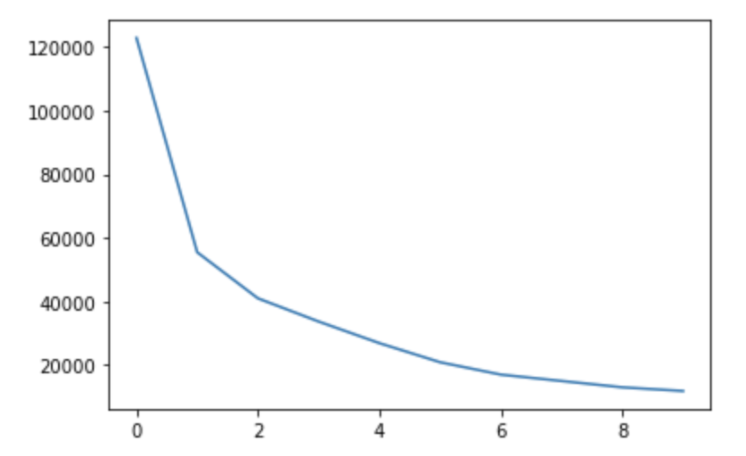
\includegraphics[scale=.8]{figure4.png}\\

\textbf{Figure 4:} WCSS versus K-values of clustering the downsampled data
\end{center}
\section*{Conclusion and discussion (0.5 pages)}
\section*{Reference (unlimited pages)}


\end{document}
